\renewcommand{\FileName}{logistic1}
\begin{frame}
  \frametitle{Logistic regression models}
  \begin{block}{\large\bfseries Response variable}<1->
      \begin{itemize*}
	   \item Binary response: success/failure, vote: yes/no
	   \item Binomial data: $x$ successes in $n$ trials (grouped data)
	   \item Ordinal response: none < some < severe depression
	   \item Polytomous response: vote Liberal, Tory, NDP, Green
      \end{itemize*}
  \end{block}
  \begin{block}{\large\bfseries Explanatory variables}<2->
      \begin{itemize*}
	  \item Quantitative regressors: age, dose
	  \item Transformed regressors: $\sqrt{\mathrm{age}}$, log(dose)
	  \item Polynomial regressors: age$^2$, age$^3$, $\cdots$
	  \item Categorical predictors: treatment, sex
	  \item Interaction regessors: treatment $\times$ age, sex $\times$ age
	  \end{itemize*}
  \end{block}
\end{frame}

\subsection{Binary response}
\begin{frame}
  \frametitle{Logistic regression models: Binary response}
  \begin{itemize*}
	\item For a binary response, $Y \in (0,1)$, want to predict $\pi = \Pr(Y=1 \given x)$
	\item Linear regression will give predicted values outside $0 \le \pi \le 1$
	\item Logistic model:
	\begin{itemize*}
	  \item $\logit ( \pi_{i}) \equiv \log [ \pi / (1 - \pi)]$ avoids this problem
	  \item logit is interpretable as ``log odds'' that $Y=1$
	\end{itemize*}
	
	\item Probit (normal transform) model $\rightarrow$ similar predictions, but is less
	interpretable
 \begin{center}
  \includegraphics[width=.4\dispwidth,clip]{fig/logitfn}
 \end{center}
  \end{itemize*}

\end{frame}

\begin{frame}
  \frametitle{Logistic regression models: Binary response}
Quantitative predictor: Linear and Logit regression on age
  \begin{itemize*}
	\item Except in extremes, linear
and logistic models give similar predicted values
	\end{itemize*}
\begin{center}
   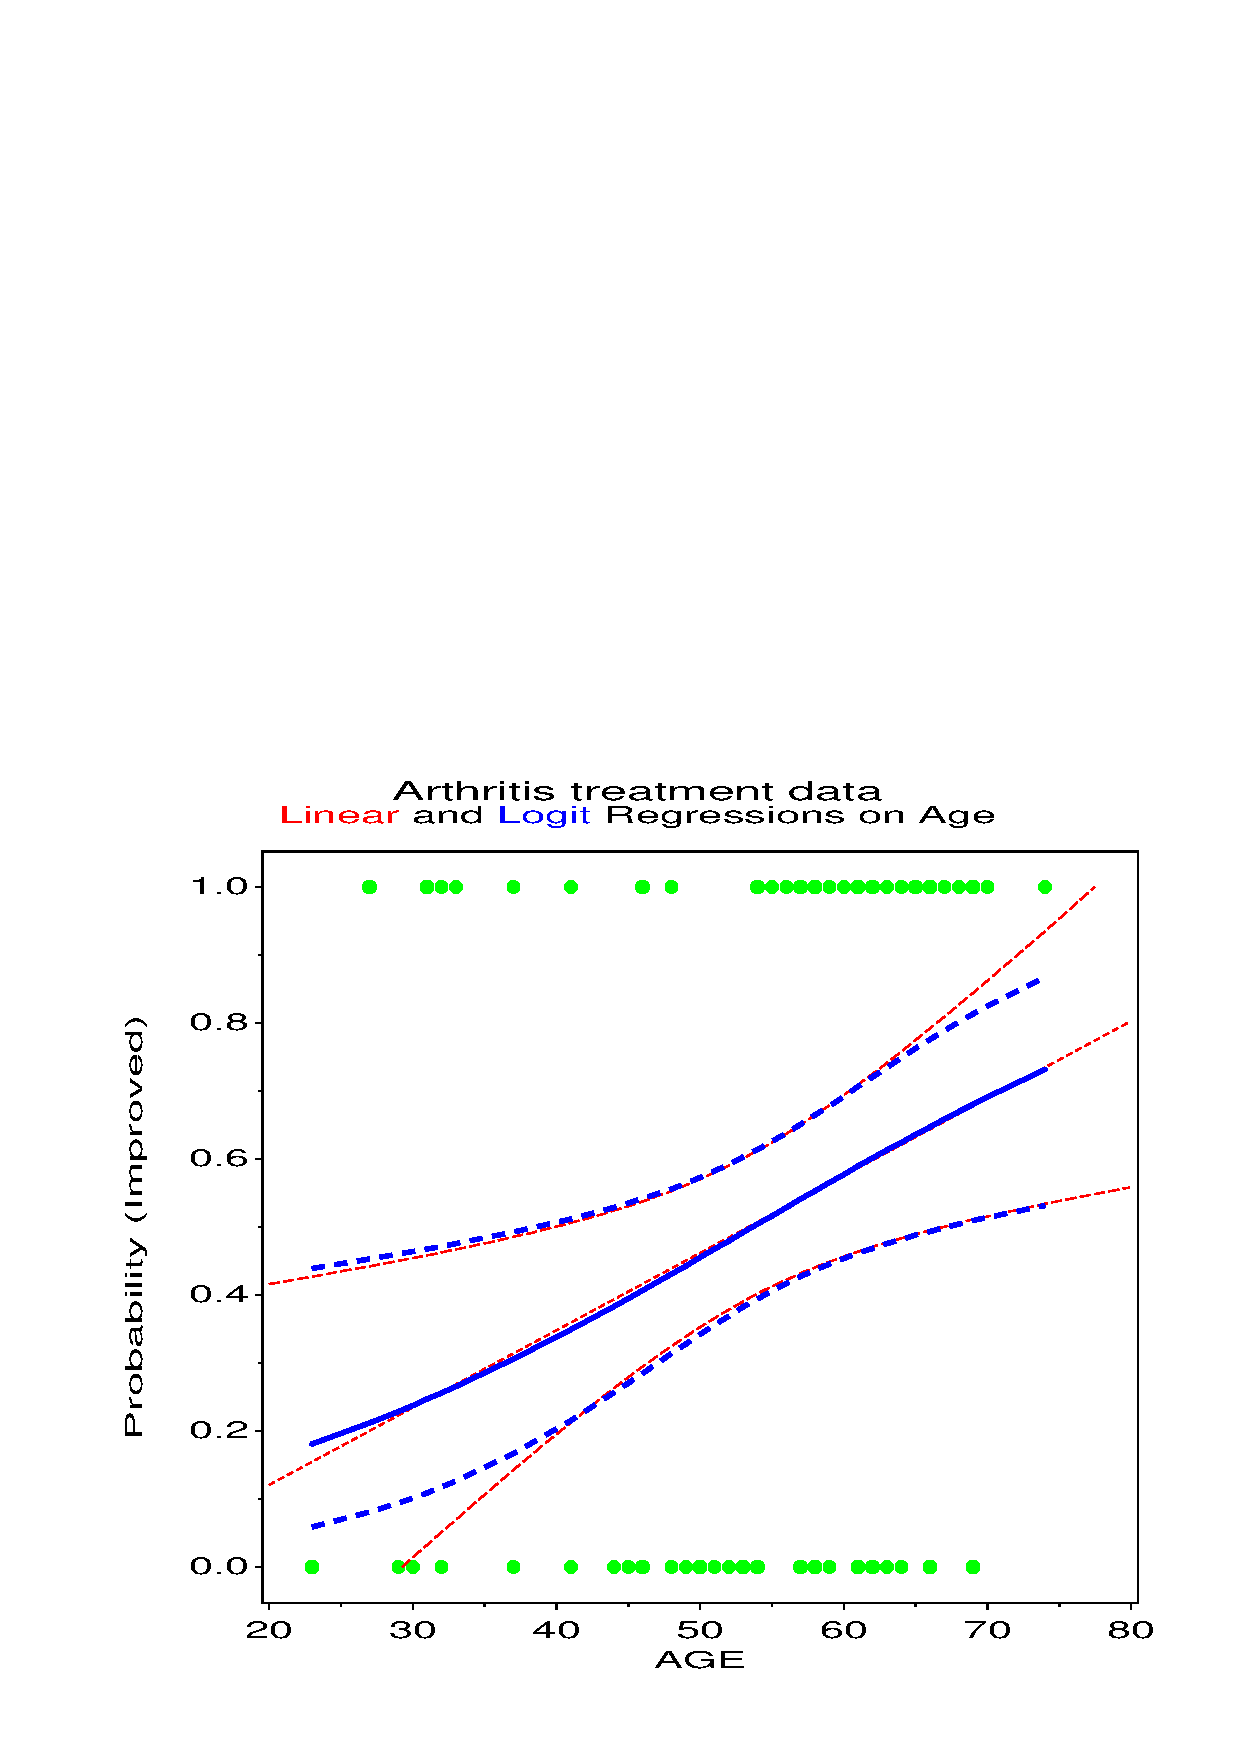
\includegraphics[height=0.7\textheight]{fig/logist1c1}
\end{center}

\end{frame}

\begin{frame}
  \frametitle{Logistic regression models: Binary response}
  \begin{itemize}[<+->]
	\item For a binary response, $Y \in (0,1)$, 
	let 
	\vec{x} be a vector of $p$ regressors, and  
	$\pi_i$ be the probability, $\Pr (Y=1 \given \vec{x})$. 
	\item The logistic regression
	model is a linear model for the \emph{log odds}, or \emph{logit}
	that $Y=1$, given the values in \vec{x},
\begin{eqnarray*}
  \logit ( \pi_{i}) \equiv \log \left( \frac{\pi_i}{1 - \pi_i}  \right)
   &=& \alpha + \vec{x}_{i}\trans \,  \vec{\beta} \\ % \label{eq:logisr}
   &=& \alpha + \beta_1 x_{i1} + \beta_2 x_{i2} + \cdots + \beta_p x_{ip}
   \nonumber
\end{eqnarray*}
	\item An equivalent (non-linear) form of the model may be specified for
	the probability,  $\pi_i$, itself,
\begin{equation*}
    \pi_i = {\{ 1 + \exp ( -[\alpha + \vec{x}_{i}\trans \,  \vec{\beta} ] ) \}}^{-1}
\end{equation*}

	\item The logistic model is a \emph{linear model} for the log odds, but also a
	\emph{multiplicative} model for the odds of ``success,''
\begin{equation*}
\frac{\pi_i}{1 - \pi_i} = \exp( \alpha + \vec{x}_{i}\trans \,  \vec{\beta} )
   = \exp(\alpha) \exp ( \vec{x}_{i}\trans \,  \vec{\beta} )
\end{equation*}
so, increasing $x_{ij}$ by 1 increases $\logit ( \pi_{i})$ by $\beta_j$,
and multiplies the odds by $e^{\beta_j}$.
%	\item Other ``link functions,'' transforming the probability, $\pi_i$,
%	to the ``linear predictor'' are possible (probit, complementary log-log)   
  \end{itemize}
\end{frame}

